\section{Completion Plan}
\label{sec:completion-plan}
In this section, a completion plan outlines all of the remaining work to be completed by the end of the project to achieve the technical objectives. The completion plan aligns with the schedule presented in the sprint plan shown in Appendix \ref{app:sprintplan} and the Gantt chart shown in Appendix \ref{app:ganttChart}. The target completion dates for each objective are included in Table \ref{tab:objectives}.

\subsection{Mapping \& Localisation}
Real time mapping and localisation is the first objective to be completed and is targeted to be done by the end of the third sprint on 18$^{th}$ June. Implementing a mapping and localisation capability necessitates hardware upgrades due to the drastic increase in required processing power for real time point cloud processing. A suitable option is to replace the Jetson Nano primary controller with a Jetson Orin NX 8GB which already in the process of being purchased. Additionally, to reduce cumulative errors involved with only using LiDAR data for SLAM, installing an IMU on the robot will be investigated. The team will begin integrating the F-LOAM open-source package with the data from the LiDAR and subsequently determine the robot's ability to perform SLAM. A specific focus of using F-LOAM is to accelerate the computational speed using the Jetson's powerful GPU. After SLAM is implemented, the robot will be tested in a controlled environment and the point cloud maps will be analysed to determine if they accurately represent the environment. To assess the algorithm's accuracy, its ARE and ATE will be determined.

\subsection{Autonomous Navigation}
Autonomous navigation encapsulates path planning as well as obstacle detection and avoidance. Due to a closely-coupled relationship between path planning and obstacle avoidance, these objectives will be developed simultaneously during the fourth and fifth sprint.

The first steps in obstacle detection rely on LiDAR point cloud preprocessing which is done by the SLAM algorithm. Thus, the obstacle detection algorithm will be implemented after SLAM implementation. Throughout the obstacle detection development process, iterative experimentation will be conducted in a controlled test environment with obstacles. This is to ensure that no premature optimisations excessively limit the algorithm's effectiveness. Following implementation and optimisation of the algorithm, true positive and false negative detection rates will be determined in the Naracoorte Caves. Much like obstacle detection is dependent on SLAM, pathfinding is dependent on obstacle detection. During implementation of the pathfinding algorithm, iterative testing will occur to identify changes which negatively impact its success rate. OB4 and OB2 will be considered completed when the prototype successfully navigates an obstacle-laden test course.

\subsection{Dynamic Gait Optimisation}
The implementation of a dynamic gait optimisation does not initially necessitate any additional hardware and will be implemented by setting up ROS topics for messages to be published about the motor's current draw. A control algorithm will subscribe to this topic and relate the current draw of each motor to its torque. Furthermore, a correlation between terrain and motor torque will be determined by testing the robot on a range of different surfaces and observing the motor torque. Ideally the control algorithm will automatically switch gaits depending on the torque experienced by each motor. If a torque level becomes too high it will indicate that the gait should be changed and if a drop in torque is observed then the gait change was successful. This control algorithm will be integrated with the existing OpenSHC package currently used by the robot.

\subsection{Development \& Debugging}
The key feature that will improve the software debugging process is the ability to transmit data to and from the robot during its operation. This capability will allow for the user to get a real time display of the map as it is produced by the LiDAR scanner (OB5). The capability will not be able to be used inside the cave environment due to signal limitations in such an environment, hence it serves purely to improve software development. The DroneDeploy software will be utilised to fulfill this capability. The DroneDeploy software allows for data communication and digital mapping through cloud-based software (Capterra 2023). A DroneDeploy license is in the process of being obtained for use by the 2023 CaveX team. To allow for this software to be used, the WiFi module shown in Appendix \ref{app:wifi-module} will be installed into the Jetson's carrier board. This module will facilitate network communication between the robot and a connected computer.

\subsection{Summary}
The progress of each technical objective is summarised in Figure \ref{fig:progress-bars}. The work needed to implement each of the technical objectives has been extensively researched and appropriate algorithms have been selected for specific objectives. Hence, progress has been made towards every one of the objectives. Localisation and mapping (OB1) has slightly more progress as procurement of new hardware has begun which represents a major milestone in achieving this objective. More progress has also been made on a gait control system (OB3) through preliminary testing that has been undertaken to identify gait effectiveness for inclined and declined surfaces.

\begin{figure}[H]
    \centering
    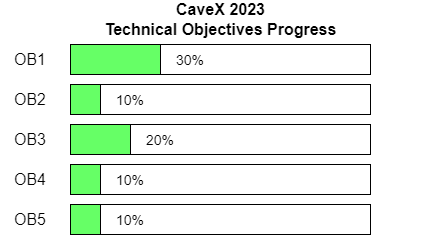
\includegraphics[scale=0.8]{images/progress_bars.png}
    \caption{CaveX 2023 technical objectives progress}
    \label{fig:progress-bars}
\end{figure}